\section{Convolutional Neural Network}
The goal of today lecture (and this section) is to being able to work with images. As said before, an image we reasonable size yields a huge vector, thus a huge amount of parameters in an MLP. Therefore we need a way to '\textit{reduce}' the size of this vector will still keeping as much information as possible. To do so we can first see the fact that small image regions have similar property (colour, \ldots) and therefore should not be processed independently. Another important thing that we need when treating images is that a translation should not affect the results. Using all of those, can we reduce the number of parameters and improve robustness?\\


\begin{parag}{CNN}
    To do so, we will introduce \important{Convolutional Neural Network} (CNN) model and its different types of layers. We will also introduce the idea of transposed convolutions for fully convolutional networks.
\end{parag}

\begin{parag}{Convolutional Layer}
    Normally if we recall the scalashop lab from cs-214, we have already seen what convolution is. The goal was to use a kernel which took as input all the neighbouring pixels and use them to output one pixel. Here this is what we will do, we will take square of input neurons and output only one neurons onto the next hidden layer. And as in cs-214, the parameters are shared across different spatial locations, meaning that the 'loop' still goes parameter by parameter (not by grid of parameters).\\
	$ $\\
	Note that each convolutional output is passed in an activation function. So, in fact,  we have 
	\begin{center}
	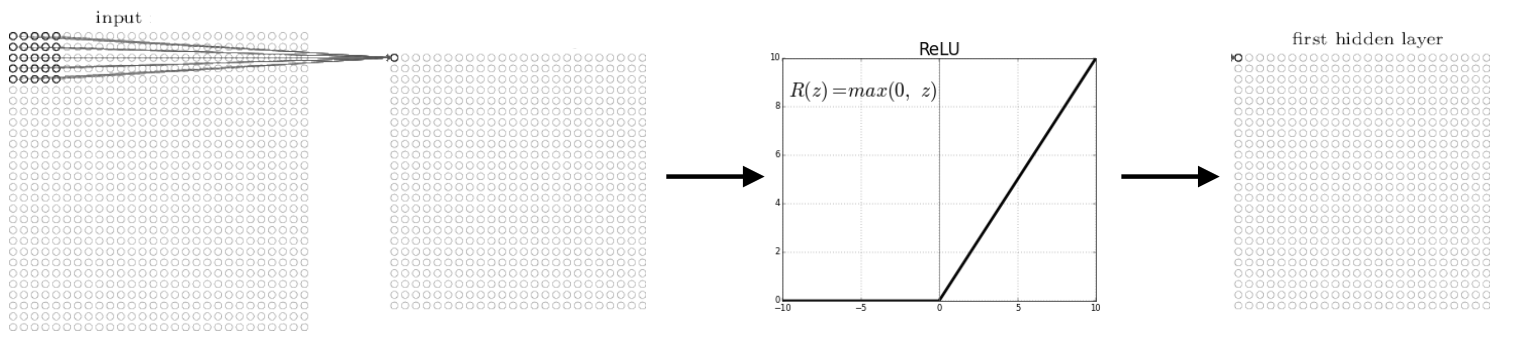
\includegraphics[scale=0.2]{screenshots/2026-04-28.png}
	\end{center}
	We can then use multiple filters to create multiple channels (3 in the example below). As in MLP each filter has its own set of learnable parameters (in the example, we have 3 $5 \times 5$ filters, i.e., 75 learnable parameters)
	\begin{center}
	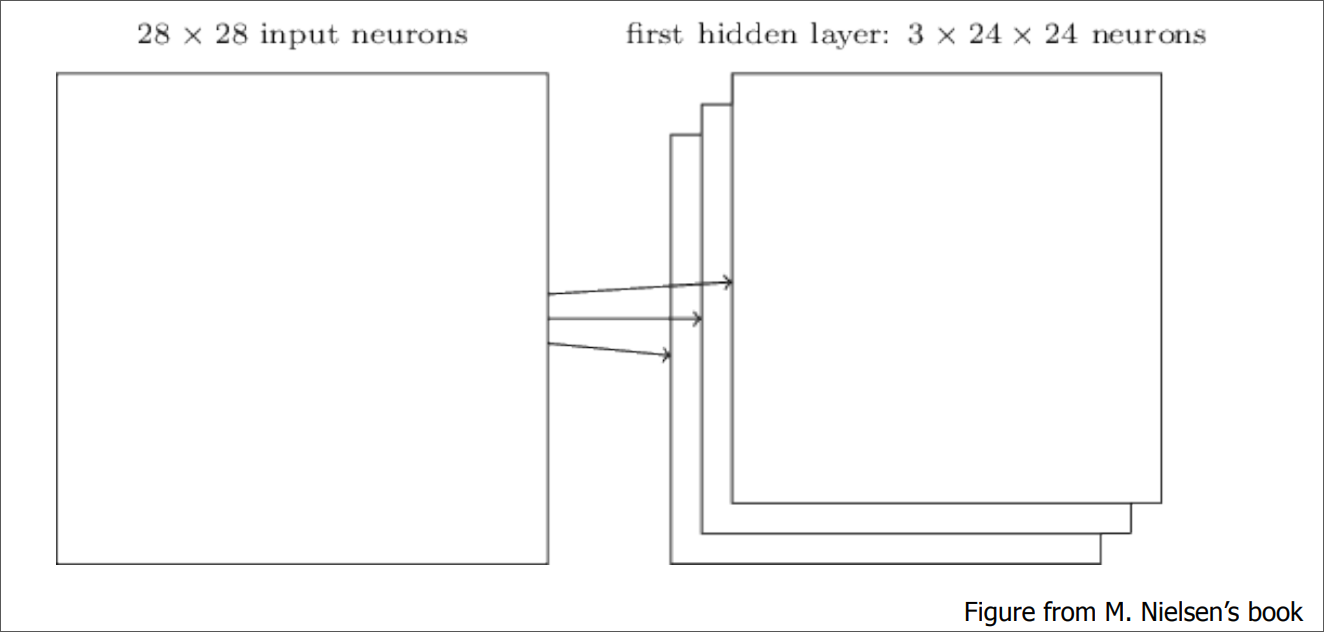
\includegraphics[scale=0.2]{screenshots/2026-04-28_1.png}
	\end{center}
\end{parag}

\begin{parag}{Pooling layer}
    This is nice, but how do we even choose what the output of the convolution is? How do we go from local information to a more global representation? There exists different pooling strategies:
	\begin{itemize}
	    \item Max pooling
	    \item Average pooling
	\end{itemize}
	Using that, we can stack these operations together and then stack multiple \important{block} of such operations. 
	\begin{subparag}{Remark}
	    \begin{itemize}
	        \item The number of channels can vary (below: first 3, then 6)
	        \item The size of filters can vary (below: first 5 $\times 5$, then $3 \times 3$)
	    \end{itemize}
	\end{subparag}
	\begin{center}
	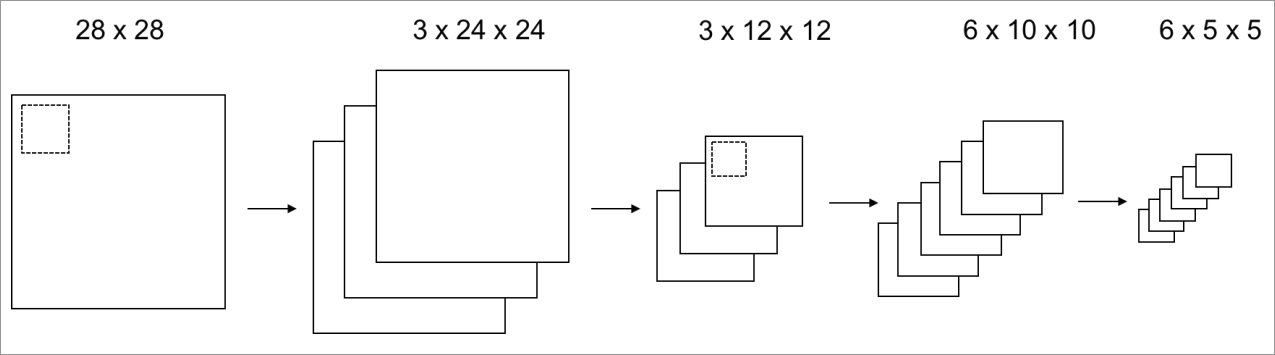
\includegraphics[scale=0.3]{screenshots/2026-04-28_2.png}
	\end{center}
\end{parag}


\begin{parag}{Padding}
    To be able to center the convolution kernel on the boundary locations, padding extends the input. This can be done by mirroring or copying the boundary values.
	\begin{center}
	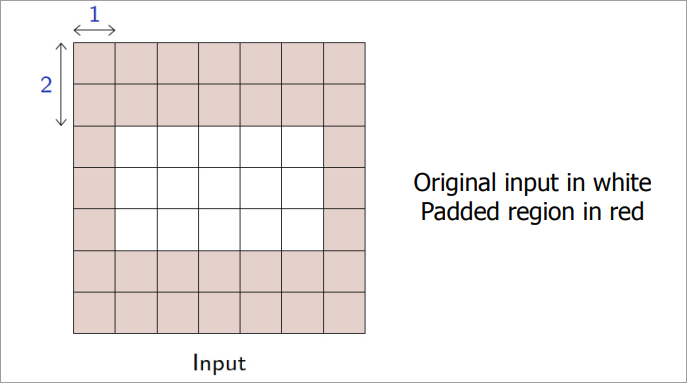
\includegraphics[scale=0.3]{screenshots/2026-04-28_3.png}
	\end{center}
\end{parag}


\begin{parag}{Convolution Stride}
    In a standard convolution, the filter is shifted pixel by pixel (as said before). The can be made larger by increasing the stride.\\
	$ $\\
	Having a larger stride gives us less parameters, the output layer will be smaller but at the cost of information.
\end{parag}


\begin{parag}{Output}
    This is nice, but what should we actually output? In general, we usually want to output a vector e.g.,
	\begin{itemize}
	    \item A vector of class probabilities for classification
	    \item A vector of 3D joint coordinates for human pose estimation
	\end{itemize}
	This can be achieved by appending fully connected layer(s). This requires vectorizing the last convolutional output first ($3 \times 12 \times 12 \to 432$-dimensional vector). Inspired by the fact that data normalization can help, several layers have been developed to normalize the feature maps, these layers include:
	\begin{itemize}
		\item Batch normalization (Ioffe \& Szegedy, ICML 2015)
	    \item Layer normalization (Ba et al., 2016)
	    \item Instance normalization (Ulyanov et al., 2016)
		\item Group normalization (We \& He, 2018)
	\end{itemize}
	
	\begin{center}
	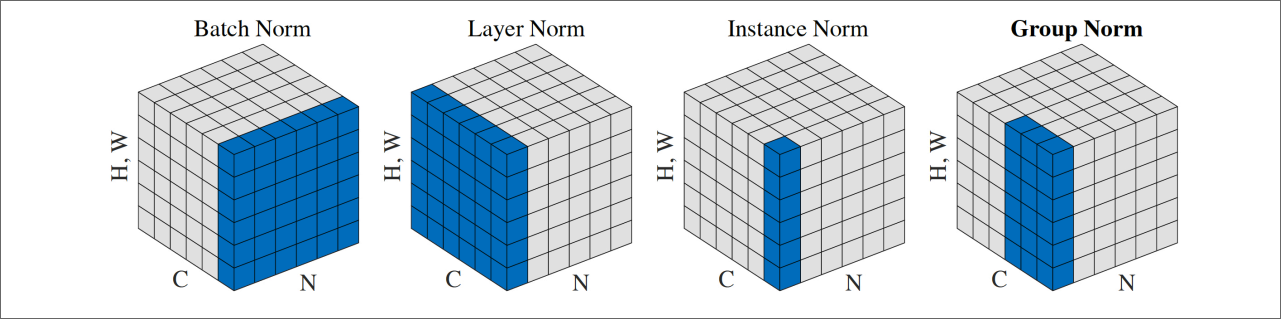
\includegraphics[scale=0.3]{screenshots/2026-04-28_4.png}
	\end{center}
	$N$ is the number of samples in a mini batch and $C$ is the number of channels; $\left(H, W\right)$ is the size of the feature map.
\end{parag}

\begin{parag}{CNN: Learning}
    Learning the weights of the CNN layers is done in the same manner as for MLPs, we use stochastic gradient descent with mini batches. As we need derivative to do so, we will still use backpropagation in order to compute those.\\
	$ $\\
	The gradient of pooling layers depends on the strategy:
	\begin{itemize}
		\item For average pooling, the gradient is backpropagated to all neurons used during pooling
		\item For max pooling, the gradient is backpropagated only to the neuron that corresponded to the maximum value
	\end{itemize}
	And we will also use all the techniques we have used before such as SGD with momentum, adaptive learning rates, Early stopping weight decay, dropout, \ldots
\end{parag}


\begin{parag}{CNN: Interpretation}
    A CNN can be thought of as jointly learning the data representation and the classifier (or regressor)
	\begin{center}
	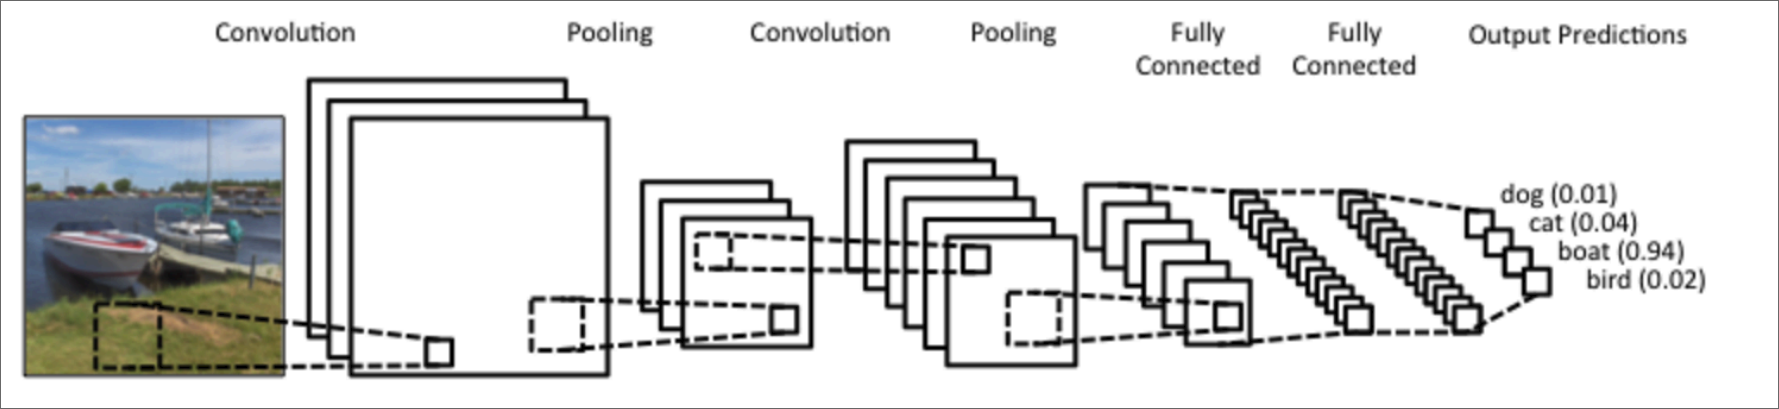
\includegraphics[scale=0.3]{screenshots/2026-04-28_5.png}
	\end{center}
	What we mean by that is that in a traditional pipeline, we separate two steps:
	\begin{itemize}
	\item Feature engineering (representation), We manually design how to turn raw data into useful numbers.
	\item Classifier/ regressor: We feed those features into a model (e.g., logistic regression, SVM)
	\end{itemize}
	The pipeline is:
	\begin{align*} 
		\begin{center}
		    \text{raw image} \to \text{handcrafted features} \to \text{classifier}
		\end{center}
	\end{align*}
	With CNN, this separation disappears, The network learns both parts simultaneously
	\begin{itemize}
	    \item Early layers learn \important{low-level} representation (edges, textures)
	    \item Middle layers learn \important{patterns} (shapes, parts of objects)
	    \item Deep layers learnt \important{semantic} (faces, cars, etc.)
	    \item Final layers act as the \important{classifier/regressor}
	\end{itemize}
	The pipeline becomes
	\begin{align*} 
		\text{ raw image } \to \text{ learned feature } \to \text{ prediction}
	\end{align*}
	Crucially, the features are not fixed, they are optimized \important{together} with the final objective\\
	$ $\\
	The network alone is saying '\textit{I will invent the features that make my classification easiest}'
	
\end{parag}



\begin{parag}{Standard architecture}
    There exists a lot of different architecture here is a couples:
	\begin{subparag}{LeNet-5}
	   \begin{center}
	   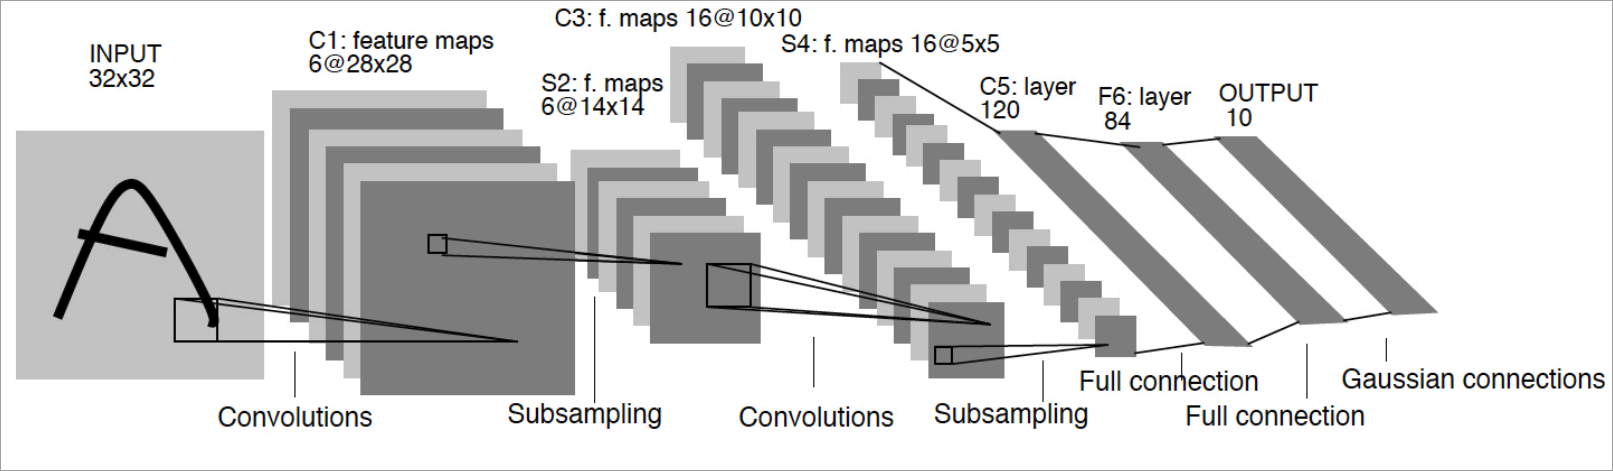
\includegraphics[scale=0.15]{screenshots/2026-04-28_6.png}
	   \end{center} 
	\end{subparag}
	\begin{subparag}{AlexNet}
	    \begin{center}
	    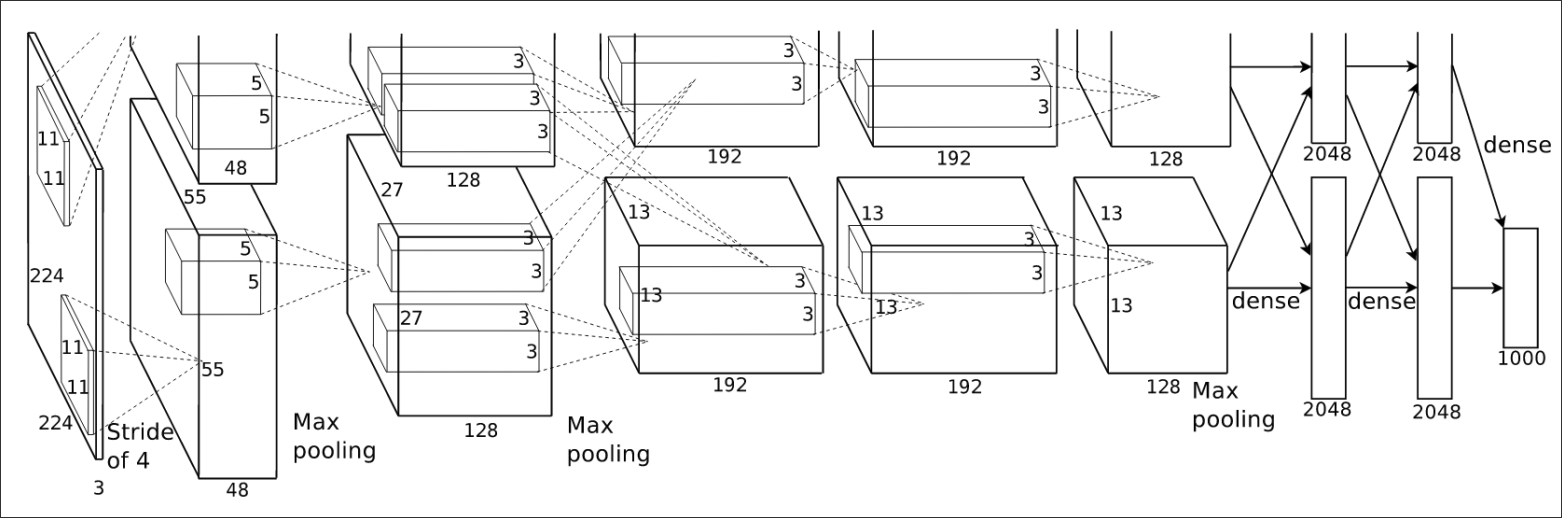
\includegraphics[scale=0.15]{screenshots/2026-04-28_7.png}
	    \end{center}
	\end{subparag}
	\begin{subparag}{VGG}
	    \begin{center}
	    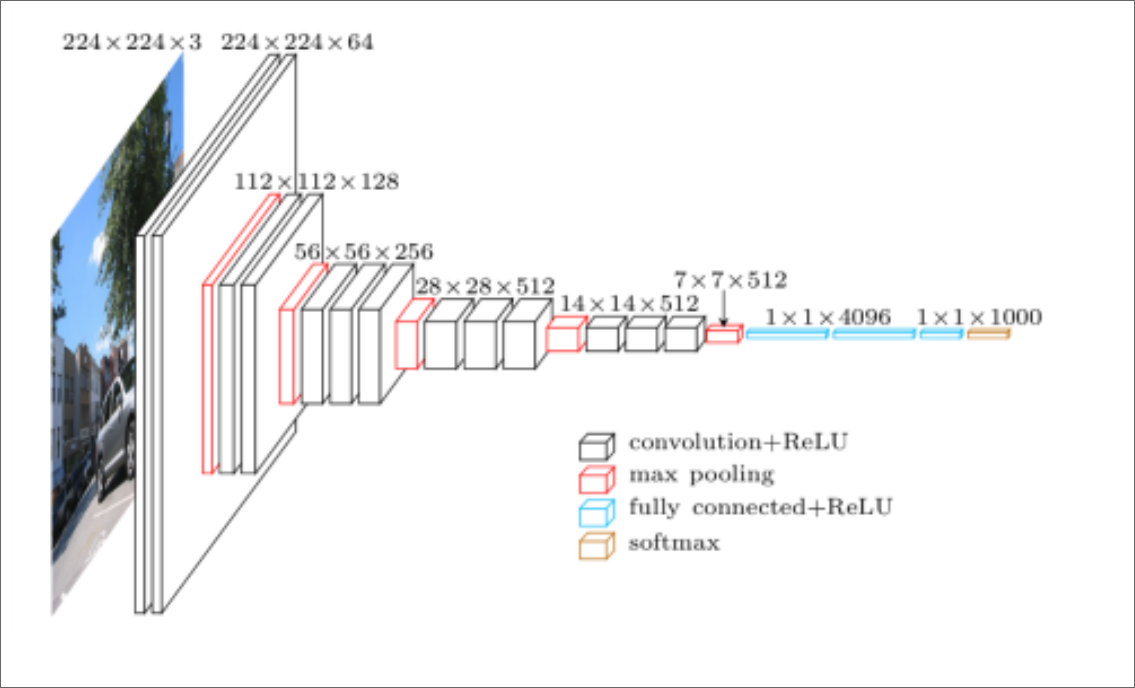
\includegraphics[scale=0.15]{screenshots/2026-04-28_8.png}
	    \end{center}
	\end{subparag}
	The standard architecture here is \important{ResNet}
	\begin{subparag}{ResNet}
		\begin{center}
			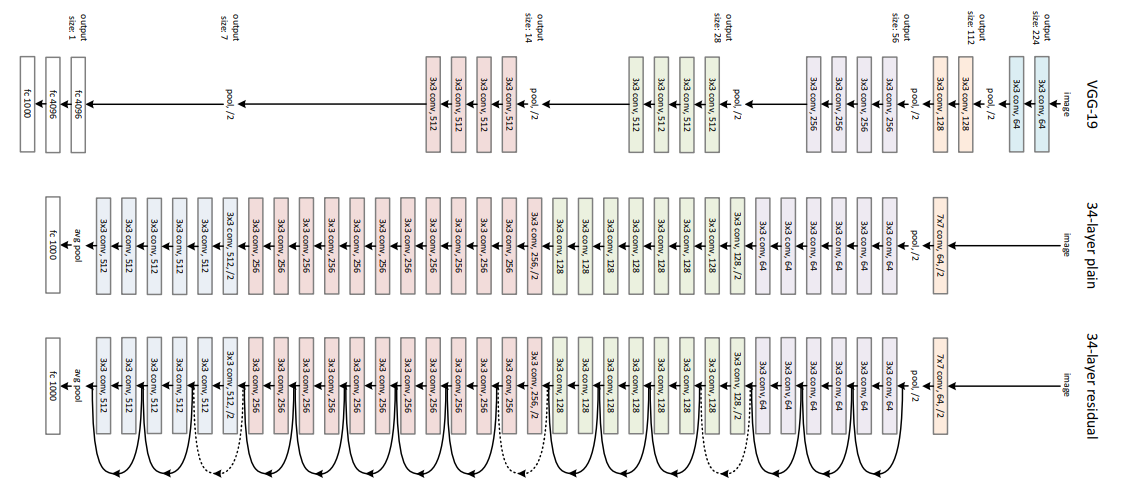
\includegraphics[scale=0.15]{screenshots/ResNet.png}
		\end{center}
		How it works is by adding to each at each layer the result of the previous layer:
	\end{subparag}
	\begin{center}
			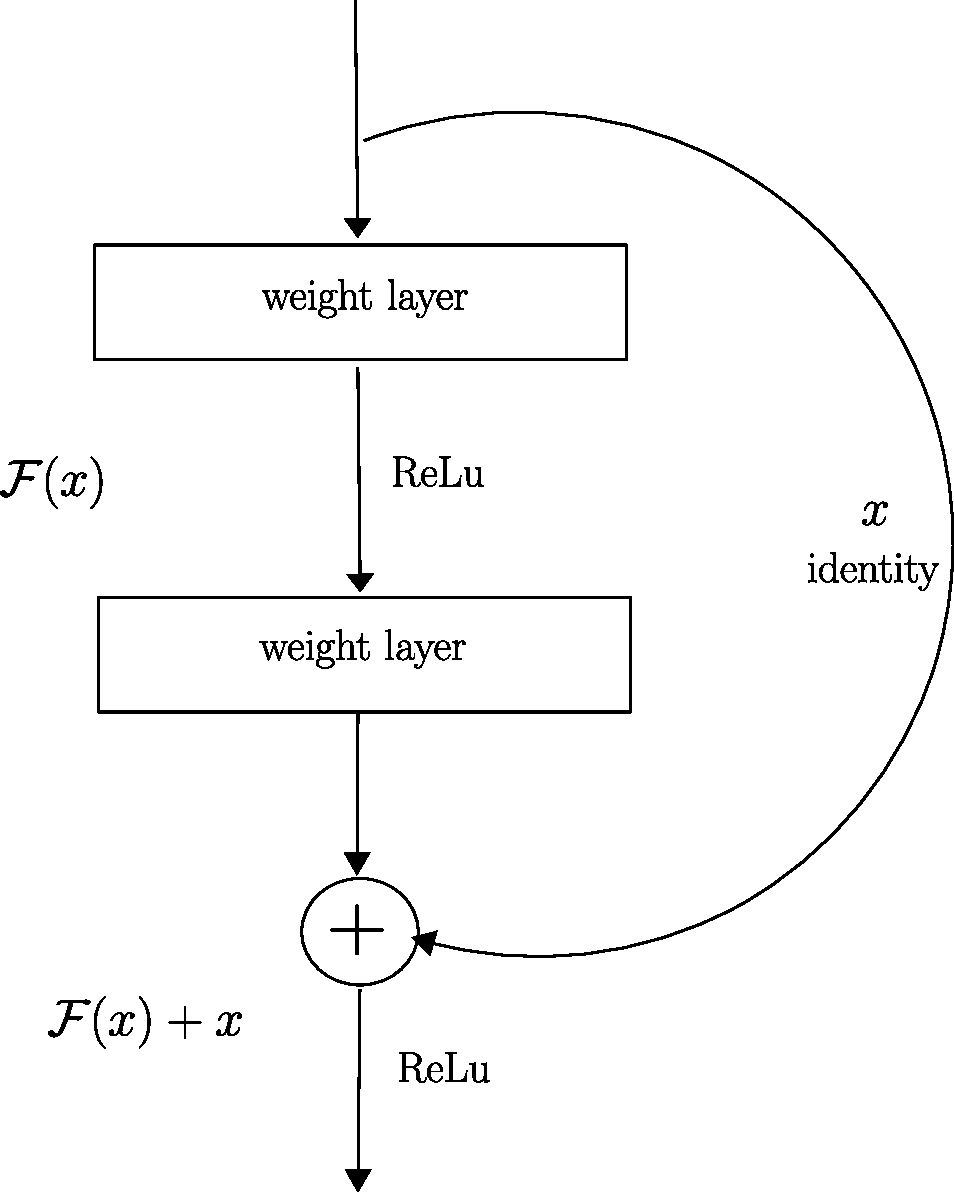
\includegraphics[width=0.35\textwidth]{figure/2026-04-28.pdf}
	\end{center}
\end{parag}

\begin{parag}{Tackling different tasks}
    When working with images, one does not necessarily want to simply classify them. For instance, semantic segmentation is the task of assigning a label to every pixel in the input image
	\begin{center}
	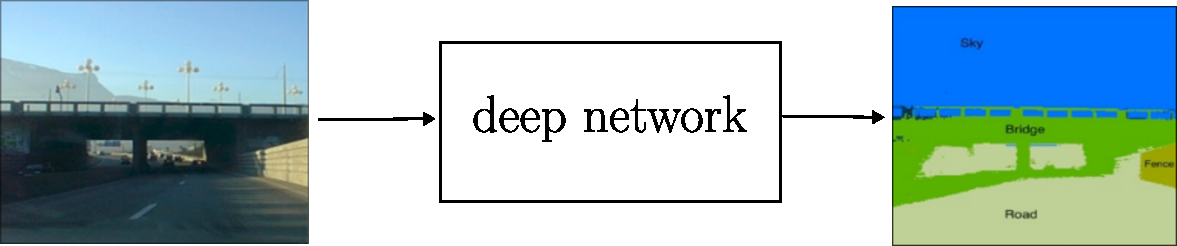
\includegraphics[width=0.8\textwidth]{figure/2026-04-28_1.pdf}
	\end{center}
\end{parag}
\begin{parag}{CNNs for semantic segmentation}
    However with the semantic segmentation as with convolutions and pooling layers the size of the feature maps decreases at every layer, with the operations seen before, we have no way of increasing this size back to the original resolution.\\
	$ $\\ We have found a way to go from an image to label, but not from label to class. A solution for this is Upsampling, followed by convolutions. To do so, let us first study the 1D convolution. For instance let us have the input:
	\begin{align*} 
		\xleftrightarrow[W]{\begin{pmatrix} 1 & 4 & -1 & 0 & 2 & -2 & 1 & 3 & 3 & 1 \end{pmatrix}}
	\end{align*}
	and the Kernel:
	\begin{align*} 
		\xleftrightarrow[w]{\begin{pmatrix} 1 & 2 & 0 & -1 \end{pmatrix}}
	\end{align*}

	If we were the compute the output, this would give us:
	\begin{align*} 
		\text{Output} =  \begin{pmatrix} 9 & 0 & 1 & 3 & -5 & -3 & 6 \end{pmatrix} 
	\end{align*}
	In essence, a 1D convolution maps a vector (of dimension $W$ in this example) to dimension $W - w +1$, increasing the dimensionality can be achieved by using the transposed matrix
	\begin{align*} 
		\begin{pmatrix} w_1 & w_2 & w_3 & 0 & 0 & 0 \\ 0 & w_1 & w_2 & w_3 & 0 & 0 \\ 0 & 0 & w_1 & w_2 & w_3 & 0 \\ 0 & 0 & 0 & w_1 & w_2 & w_3 \end{pmatrix}^{T} = \begin{pmatrix} w_1 & 0 & 0 & 0 \\ w_2 & w_1 & 0 & 0 \\ w_3 & w_2 & w_1 & 0 \\ 0 & w_3 & w_2 & w_1 \\ 0 & 0 & w_3 & w_2 \\ 0 & 0 & 0 & w_3 \end{pmatrix} 
	\end{align*}
	Therefore using that on the kernel:
	\begin{align*} 
		k = \begin{pmatrix} 1 & 2 & -1 \end{pmatrix} 
	\end{align*}
	and the input 
	\begin{align*} 
		I = \begin{pmatrix} 2 & 3 & 0 & -1 \end{pmatrix} 
	\end{align*}
	The output is given as:
	\begin{align*} 
		\begin{pmatrix} 2 & 7 & 4 & -4 & -2 & 1 \end{pmatrix} 
	\end{align*}
\end{parag}

\begin{parag}{2D convolution as matrix product}
    A similar matrix representation can be obtained for 2D convolutions. This input is vectorized, e.g., by concatenating its columns. The matrix is obtained by spreading the different columns of the kernel at the matching locations 
	\begin{center}
	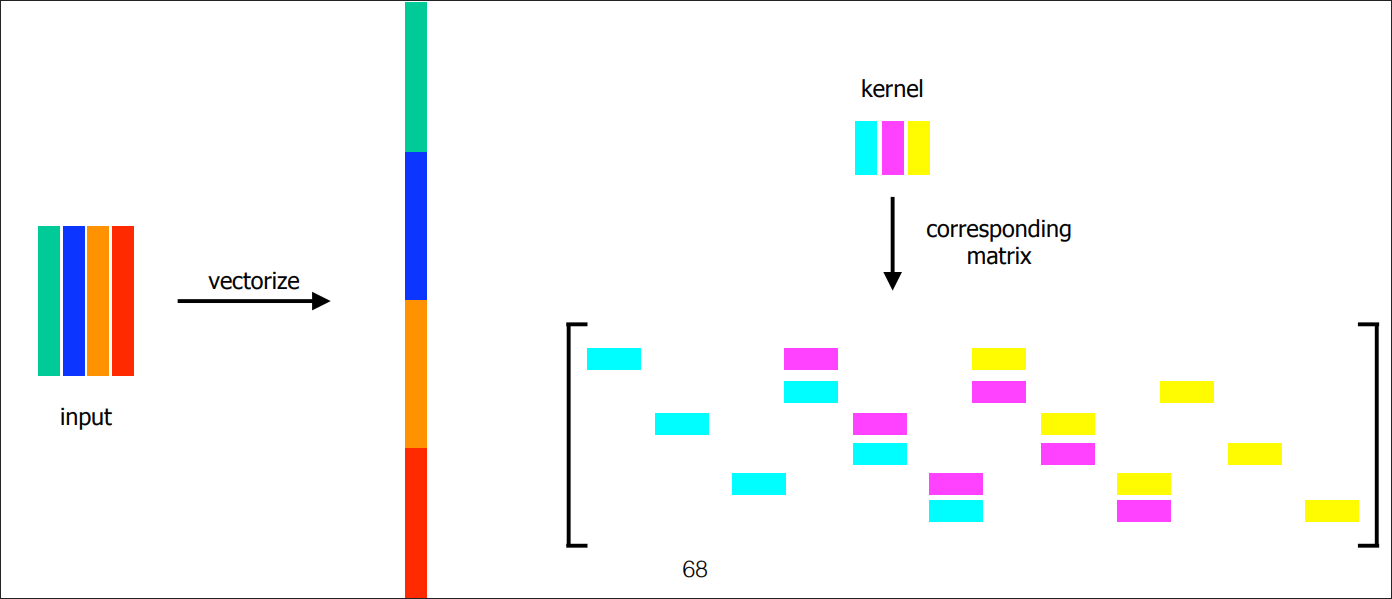
\includegraphics[scale=0.2]{screenshots/2026-04-28_11.png}
	\end{center}
\end{parag}

\begin{parag}{Fully convolutional networks}
    Stacking upsampling convolutions, or transposed convolutions, after regular ones lets us go back to the original spatial resolution.
	\begin{itemize}
	    \item For binary semantic segmentation, the output is a binary mask of the same size as the image (here overlaid on top of the input)
	    \item Ronneberger et al., U-Net: Convolutional Networks for Biomedical Image Segmentation, MICCAI 2015
	\end{itemize}
	\begin{center}
	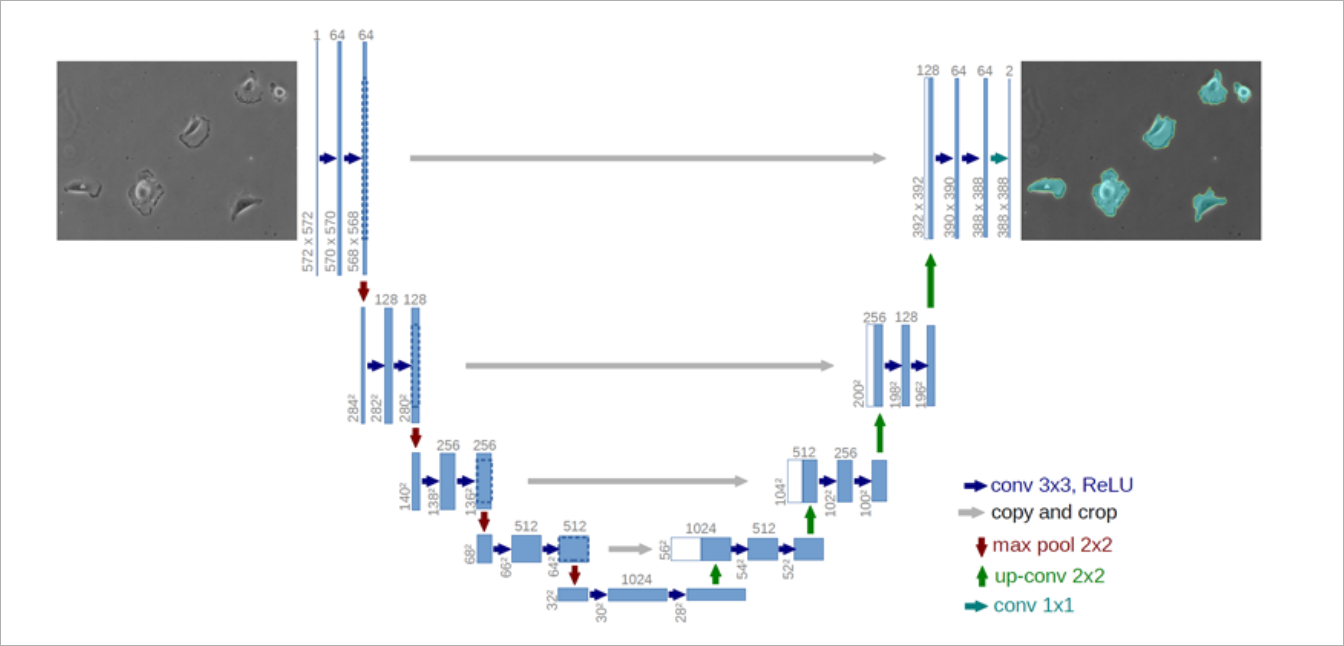
\includegraphics[scale=0.15]{screenshots/2026-04-28_12.png}
	\end{center}
\end{parag}




\begin{parag}{Deep Learning: Tricks of the trade}
    In order to have better performance and be less costly in term of performance, we can use a couple of techniques 
	\begin{itemize}
	    \item Pre-training: People often start with a standard architecture trained on ImageNet
	    \item Learning rate scheduling: Decrease the learning rate after a pre-defined number of epochs
	    \item Use a cyclic learning rate
	\begin{center}
	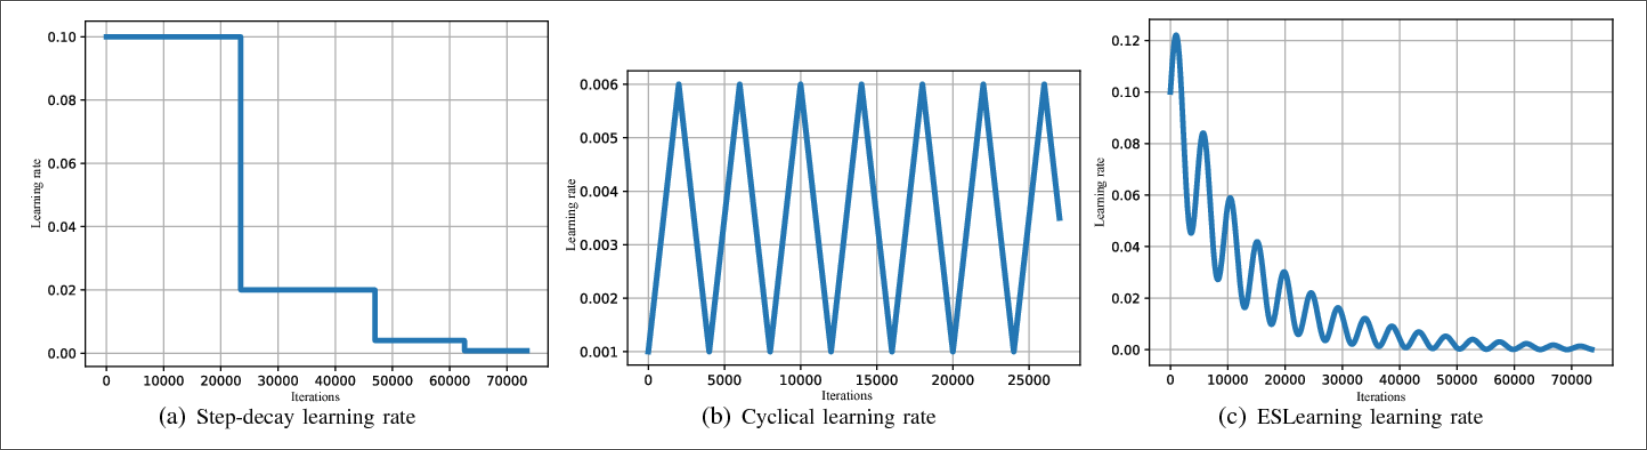
\includegraphics[scale=0.2]{screenshots/2026-04-28_13.png}
	\end{center}
\item Data augmentation
	\end{itemize}
	
\end{parag}








